\documentclass[conference]{IEEEtran}
\IEEEoverridecommandlockouts
\usepackage{cite}
\usepackage{amsmath,amssymb,amsfonts}
\usepackage{algorithmic}
\usepackage{graphicx}
\usepackage{textcomp}
\usepackage{xcolor}
\usepackage{kotex}
\usepackage{multirow}
\usepackage{booktabs}
\usepackage{array}
\usepackage{url}

\def\BibTeX{{\rm B\kern-.05em{\sc i\kern-.025em b}\kern-.08em
    T\kern-.1667em\lower.7ex\hbox{E}\kern-.125emX}}

\begin{document}

\title{GDP(Generative Digital-twin Prototyper): LLM 기반 공정 설계 자동화 및 분석 도구 연동 프레임워크}

\author{\IEEEauthorblockN{이건창}
\IEEEauthorblockA{\textit{DMC공학과} \\
\textit{성균관대학교}\\
수원, 대한민국 \\
ilsc2908@skku.edu}
\and
\IEEEauthorblockN{우홍욱\textsuperscript{*}}
\IEEEauthorblockA{\textit{소프트웨어학과} \\
\textit{성균관대학교}\\
수원, 대한민국 \\
hwoo@skku.edu}
}

\maketitle

\begin{abstract}
스마트 인더스트리(Smart Industry)의 핵심 기술인 디지털 트윈 구현을 위해서는 정교한 제조 데이터와 이를 활용한 시뮬레이션 체계가 필수적이다. 그러나 제조 현장은 비전문가가 접근하기 어려운 데이터 폐쇄성과, 전문가가 직면하는 도구 간 인터페이스 파편화라는 이중의 장벽이 존재한다. 본 논문에서는 거대언어모델(LLM)을 기반으로 두 사용자 그룹의 문제를 동시에 해결하는 GDP(Generative Digital-twin Prototyper) 프레임워크를 제안한다. GDP는 첫째, 비전문가 및 연구자가 제조 지식 없이도 제로-샷(Zero-shot)으로 연구용 모의 공정 데이터를 생성할 수 있는 환경을 제공한다. 이는 휴머노이드 등 피지컬 AI(Physical AI) 연구를 위한 가상 테스트베드로 활용 가능하다. GDP는 이를 위해 지멘스(Siemens)가 제안한 BOP(Bill of Process) 개념을 채택하여 신뢰도 높은 공정 모델링을 수행한다. 둘째, 전문가 및 개발자가 시뮬레이션이나 최적화 도구를 연동할 때 발생하는 인터페이스 구축 비용을 LLM 기반 어댑터 자동 생성 및 Auto-Repair 메커니즘을 통해 획기적으로 낮춘다. 실험 결과, 10종 제품군에 대한 제로-샷 공정 생성에서 F1 88.9\%를 달성하여 비전문가의 데이터 확보 가능성을 입증하였으며, 전문가용 도구 연동 실험에서는 Auto-Repair를 통해 실행 통과율 100\%를 확보함과 동시에 16.2\%의 `조용한 실패(Silent Failure)' 현상을 관측하여 실행 통과만으로는 불충분하며 2단계 평가가 필요함을 실증하였다.
\end{abstract}

\begin{IEEEkeywords}
Digital Twin, LLM, Manufacturing, Bill of Process, Tool Integration, Auto-Repair
\end{IEEEkeywords}

%% ============================================================
\section{서론}
%% ============================================================

스마트 인더스트리(Smart Industry) 시대의 제조 경쟁력은 물리적 공장을 가상 공간에 복제하여 사전 검증하는 디지털 트윈 기술의 완성도에 달려 있다. 디지털 트윈은 설계 단계에서의 병목 예측, 공정 최적화, 실시간 모니터링을 가능하게 하여 제조 혁신의 핵심 인프라로 자리매김하고 있다~\cite{b1}. 그러나 연구 및 개발 단계에서 디지털 트윈을 고도화하는 과정에서 두 가지 큰 장벽에 부딪히고 있다.

첫째는 \textbf{벤치마크 데이터의 부재 및 파편화}이다. 실제 제조 데이터는 기업의 핵심 보안 자산으로서 외부 공개가 엄격히 제한되어 있어, 외부 연구자가 시뮬레이션 고도화에 활용할 수 있는 신뢰도 높은 공개 데이터셋을 확보하기 어렵다.

둘째는 공정 설계와 분석 도구 간의 \textbf{인터페이스 파편화}이다. 각 분석 도구는 고유한 입출력 형식을 요구하며, 엔지니어들은 데이터 전처리와 어댑터 개발에 막대한 시간을 소비하고 있다.

이러한 장벽은 제조 도메인 지식이 부족한 \textit{비전문가}(타 분야 연구자)와, 반복적 인터페이스 개발에 과도한 노력을 소비하는 \textit{전문가}(공정 엔지니어)에게 각기 다른 방식으로 영향을 미친다. 본 연구는 이 두 가지 문제를 동시에 해결하는 GDP 프레임워크를 제안하며\footnote{소스 코드 및 실험 데이터: \url{https://github.com/lee-geon-chang/gdp}}, 다음 세 가지 연구 질문에 답한다:

\begin{itemize}
\item \textbf{RQ1}: 도메인 지식이 없는 비전문가도 LLM을 통해 제조 공정 구조를 생성할 수 있는가?
\item \textbf{RQ2}: LLM 기반 어댑터는 도구 통합 비용을 절감할 수 있는가?
\item \textbf{RQ3}: 실제 도구 파이프라인에서 LLM 기반 자동 복구(Auto-Repair)는 얼마나 신뢰할 수 있는가?
\end{itemize}

이에 대해 비전문가에게는 제로-샷 공정 설계를, 전문가에게는 자동화된 도구 연동을 제공한다. 주요 기여도는 다음과 같다:

\begin{enumerate}
\item \textit{비전문가를 위한 제로-샷 공정 설계}: 제조 지식이 부족한 사용자도 자연어 입력만으로 Siemens가 제안한 BOP 개념을 기반으로 구조적으로 완결된 공정 데이터를 생성할 수 있다. 이를 통해 생성된 모의 데이터는 휴머노이드 로봇 및 피지컬 AI(Physical AI) 학습을 위한 가상 제조 환경 구축에도 활용될 수 있다.

\item \textit{전문가를 위한 인터페이스 자동화 및 Auto-Repair}: 기존 스크립트 어댑터 자동 생성, AI 기반 분석 도구 합성, 스키마 가이드 최적화의 세 가지 연동 방식을 제공하고, 실행 중 발생하는 런타임 에러를 LLM이 자율적으로 감지\,$\cdot$\,수정하는 자가 복구 메커니즘을 구현하였다.
\end{enumerate}

%% ============================================================
\section{관련 연구}
%% ============================================================

\subsection{디지털 트윈의 표준화 및 모델링 자동화}

디지털 트윈은 물리적 자산의 가상 복제본으로, 모니터링 및 시뮬레이션을 통해 최적의 의사결정을 지원한다~\cite{b1}. 최근에는 `Digital Twin Shop-floor' 개념으로 제조 현장까지 확장되었으며~\cite{b2}, ISO 23247 표준이 4계층 아키텍처를 통해 데이터-모델 간 연결성을 강조하고 있다~\cite{b3}.

그러나 표준 모델의 현장 적용에는 여전히 높은 모델링 비용이 수반되며, 공정 모델링이 숙련된 엔지니어의 수작업에 의존하고 있다~\cite{b4}. 온톨로지 기반 접근은 신규 공정에 유연하게 대응하지 못하며~\cite{b5}, Siemens BOP는 Plant $\rightarrow$ Line $\rightarrow$ Station $\rightarrow$ Operation의 심층 계층 구조를 제안하였으나 대규모 PLM 시스템을 전제로 하여 경량 프로토타이핑에는 과도한 복잡성을 수반한다.

\subsection{거대언어모델(LLM)을 활용한 제조 지식 구조화}

최근 LLM은 비정형 텍스트로부터 논리적 구조를 추출하여 산업용 데이터로 변환하는 데 뛰어난 성과를 보이며~\cite{b6}, 제조 도메인에서의 CAPP(Computer-Aided Process Planning) 연구로 확장되고 있다~\cite{b7}. 제로-샷 추론으로 제조 시나리오를 JSON/XML 공정 명세서로 변환하는 시도가 이루어지고 있으나~\cite{b8}, 생성 공정의 세분화 수준이 프롬프트와 스키마 제약에 따라 크게 달라져 체계적 평가가 필요하다. BOP 개념에 매핑하여 시뮬레이션 도구와 연동하는 연구는 초기 단계이며~\cite{b9}, 최근에는 LLM과 디지털 트윈의 통합을 Industry~5.0 관점에서 체계적으로 조망하는 프레임워크도 제시되었으나~\cite{b16}, 실질적인 도구 연동 파이프라인까지 구현한 사례는 드물다. 본 연구는 LLM 사전 지식과 공정 모델 정제를 결합하여 하류 분석 도구와의 스키마 수준 호환성을 보장한다.

\subsection{이기종 도구 통합 및 어댑터 자동 생성 기술}

공정 설계 데이터가 시뮬레이션이나 최적화 엔진으로 전달되는 과정에서 발생하는 `인터페이스 파편화'는 디지털 트윈 구축의 최대 병목 현상이다~\cite{b10}. 하나의 BOP 데이터를 $N$개의 분석 도구에 연동하려면 각각 고유한 입출력 스키마를 가진 $O(N)$개의 어댑터를 개별 개발해야 한다. 기존에는 AutomationML이나 OPC UA와 같은 표준을 통해 데이터 교환의 자동화를 꾀했으나, 이는 주로 하위 필드의 데이터 전송에 집중되어 있어 상위 설계 단계에서의 도메인별 어댑터 개발은 여전히 필수적이다~\cite{b11}.

최근에는 LLM의 코드 생성 능력을 활용하여 서로 다른 데이터 스키마 간의 매핑 코드를 자동 합성하려는 시도가 진행 중이며~\cite{b12}, LLM의 함수 호출(function calling) 기능을 산업 워크플로에 적용하는 연구도 활발하다~\cite{b17}. 자연어 요구사항으로부터 실행 가능한 스크립트를 생성하는 가능성이 확인되었다~\cite{b13}. 그러나 런타임 오류를 시스템이 스스로 분석하고 수정하는 `Self-healing' 또는 `Auto-Repair' 메커니즘의 도입이 점차 중요해지고 있다~\cite{b14}. 최근에는 LLM이 자체 생성한 테스트를 활용한 self-debugging~\cite{b18}과 강화 학습 기반 자가 수정 학습~\cite{b19}이 제안되었으나, 제조 디지털 트윈의 도구 인터페이스에는 아직 적용된 사례가 없으며, 본 프레임워크가 이를 최초로 적용한다.

%% ============================================================
\section{제안하는 GDP 프레임워크}
%% ============================================================

GDP는 LLM 기반의 제조 공정 설계 자동화 및 분석 도구 연동 프레임워크로, Fig.~\ref{fig:overview}와 같이 두 단계로 동작한다. Step~1에서는 자연어 입력으로부터 LLM의 사전 지식을 활용하여 완전한 BOP를 생성한다. Step~2에서는 생성된 BOP를 외부 분석 도구와 자동 연동하여 설계를 고도화하며, 런타임 에러를 자가 수정하는 Auto-Repair 메커니즘이 이를 지원한다. 두 단계 모두 LLM 생성 효율과 도구 상호운용성을 위해 설계된 공정 중심(process-centric) 데이터 모델 위에서 동작하며, 이를 먼저 기술한다.

\subsection{Process-centric 공정 데이터 모델}

Siemens BOP는 Plant $\rightarrow$ Line $\rightarrow$ Station $\rightarrow$ Operation의 깊은 계층 구조를 가지나, 이를 그대로 LLM 프롬프트에 포함시키면 토큰 소모가 과도해지고 생성 정확도가 저하된다. GDP는 이 문제를 해결하기 위해 공정(Process)을 핵심 단위로 하는 평탄화된(flattened) 데이터 모델을 설계하였다.

BOP 데이터는 프로젝트 메타정보(프로젝트명, 목표 UPH)와 함께 공정 테이블(processes)을 중심 엔터티로 하고, 설비(equipments)\,$\cdot$\,작업자(workers)\,$\cdot$\,자재(materials)의 세 가지 리소스 마스터를 참조하는 구조이다. 각 공정은 고유 ID\,$\cdot$\,명칭\,$\cdot$\,사이클 타임\,$\cdot$\,선후행 관계를 가지며, 리소스는 배정(assignment) 엔터티를 통해 공정에 종속적으로 매핑된다. 즉, 하나의 공정이 어떤 설비를 사용하고, 몇 명의 작업자가 투입되며, 어떤 자재를 소비하는지가 배정 엔터티에 기록된다. 배정 엔터티는 리소스 유형\,$\cdot$\,참조 ID\,$\cdot$\,수량과 함께 \textbf{공정 중심점 기준의 상대 좌표(relative location)}를 보유한다. 리소스의 실제 3D 위치는 다음과 같이 계산된다:

\begin{equation}
\mathbf{p}_{\mathrm{actual}} = \mathbf{p}_{\mathrm{process}} + \mathbf{p}_{\mathrm{relative}}
\label{eq:coord}
\end{equation}

이 이중 좌표 체계 덕분에 공정 단위의 이동 시 하위 리소스의 좌표를 개별 재계산할 필요가 없어 레이아웃 수정 비용이 대폭 절감된다.

공정 간 선후행 관계는 임의의 분기(branching)와 합류(merging)를 허용하는 DAG(Directed Acyclic Graph) 구조로 표현되며, 순환 참조는 실시간으로 탐지\,$\cdot$\,차단된다. 병렬 처리(parallel processing)는 동일 공정의 복수 인스턴스로 표현되어, 각 병렬 라인의 독립적 편집과 3D 렌더링을 지원한다. 설비는 로봇(robot), 기계(machine), 수동 스테이션(manual\_station)의 세 유형으로 분류되며, 작업자가 배치된 공정에는 반드시 수동 스테이션이 동반되어야 하는 물리적 제약조건이 생성 시 자동으로 부과된다.

\subsection{시스템 개요}

GDP는 브라우저 기반 통합 환경으로, Fig.~\ref{fig:overview} 상단과 같이 세 개의 동기화된 패널로 구성된다. \textbf{BOP 테이블(좌측)}은 공정, 사이클 타임, 배정된 리소스를 스프레드시트 형태로 표시하며 직접 편집이 가능하다. \textbf{3D 레이아웃(중앙)}은 공정 흐름과 리소스 배치를 3차원 공간에서 시각화하며, 사용자는 모든 객체에 대해 이동, 회전, 크기 조절을 마우스로 수행할 수 있다. \textbf{AI 어시스턴트(우측)}는 자연어 채팅 인터페이스로, 사용자의 명령을 LLM에 전달하여 BOP 생성, 수정, 질의를 처리한다. LLM 제공자는 교체 가능(pluggable)하며 다양한 모델군을 지원한다. 세 패널은 양방향으로 동기화되어, 어느 패널에서든 수정 사항이 즉시 나머지 패널에 반영된다.

\begin{figure}[!t]
\centering
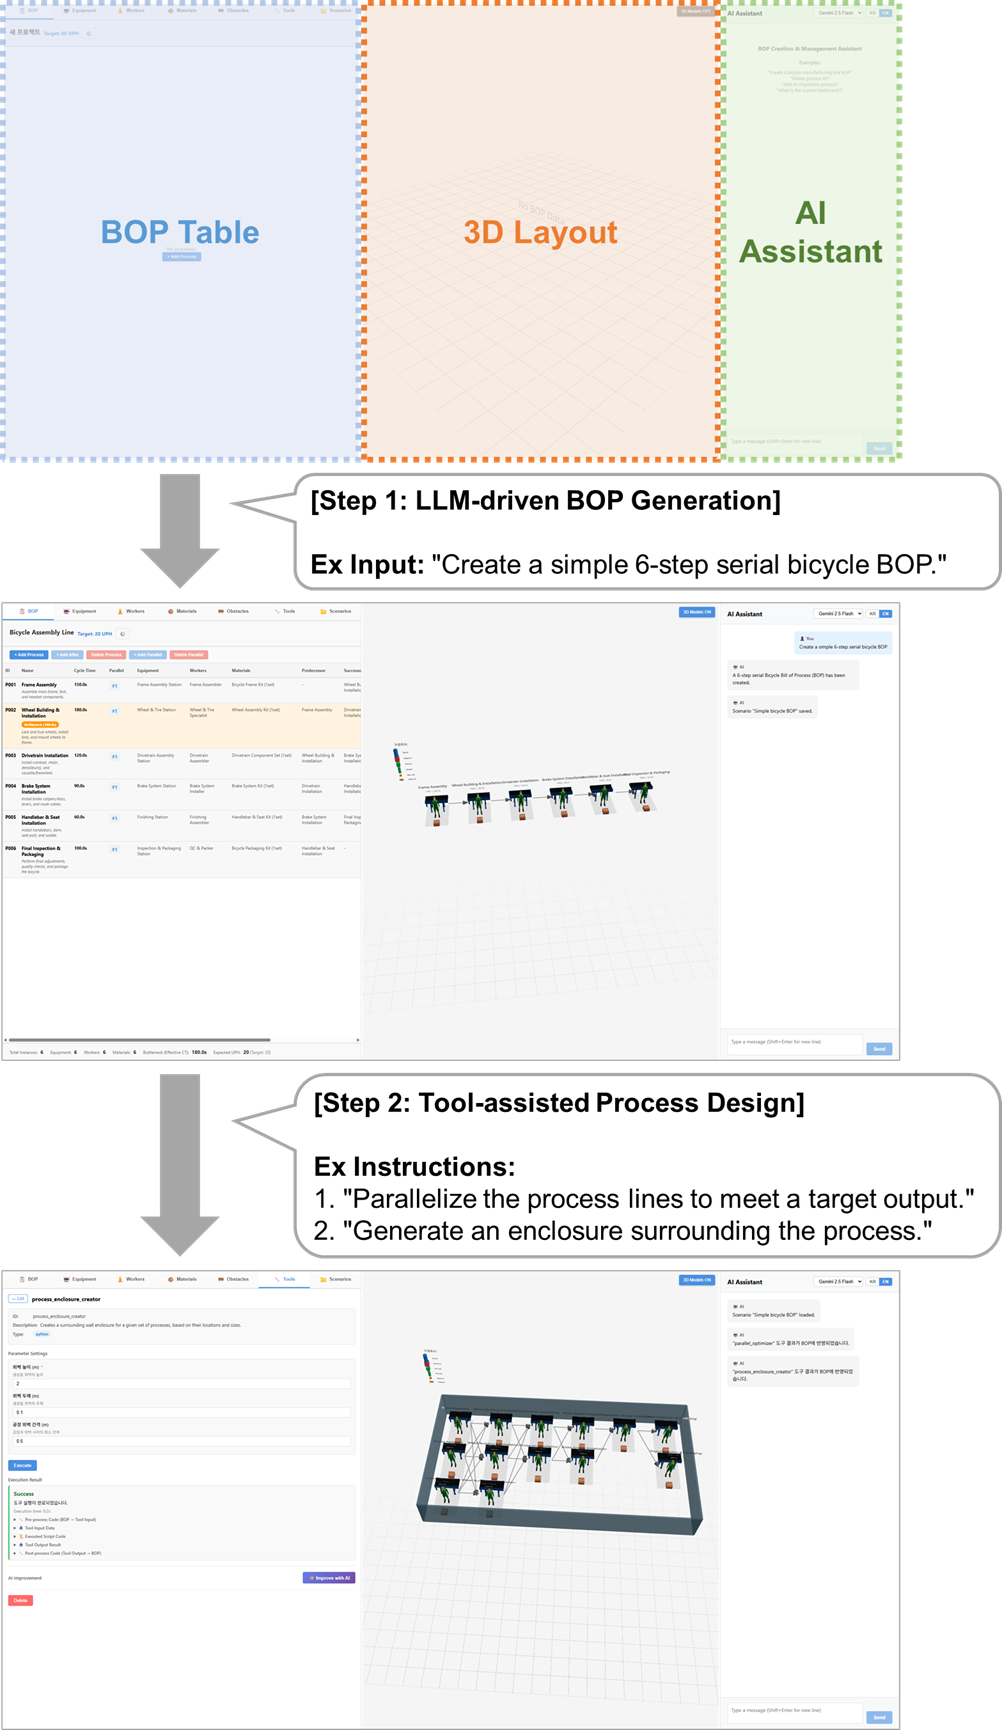
\includegraphics[width=\columnwidth]{fig1.png}
\caption{GDP 시스템 개요. 상단: BOP 테이블, 3D 레이아웃, AI 어시스턴트로 구성된 통합 화면. Step~1: LLM 기반 BOP 생성. Step~2: 외부 도구 연동 및 Auto-Repair를 통한 설계 고도화.}
\label{fig:overview}
\end{figure}

\subsection{LLM 기반 BOP 생성 (Step~1)}

Fig.~\ref{fig:overview}의 Step~1은 자연어로부터 시뮬레이션 가용한 공정 설계를 생성하는 과정을 보여준다. 예를 들어 사용자가 ``\textit{Create a simple 6-step serial bicycle BOP}''라고 입력하면, 시스템은 아래의 파이프라인을 자동 수행한다.

자연어 입력 $q$, 출력 스키마 $\mathcal{S}$, 도메인 제약조건 $\mathcal{C}$가 주어질 때, Step~1의 파이프라인은 다음과 같이 정의된다:
\begin{equation}
B = \mathrm{Validate}\bigl(\mathrm{LLM}(q,\;\mathcal{S},\;\mathcal{C})\bigr)
\label{eq:step1}
\end{equation}
여기서 $B = (\mathcal{P}, \mathcal{E}, \mathcal{W}, \mathcal{M}, \mathcal{A})$는 공정 집합 $\mathcal{P}$, 설비 $\mathcal{E}$, 작업자 $\mathcal{W}$, 자재 $\mathcal{M}$, 배정 $\mathcal{A}$로 구성된 BOP이다. 먼저 사용자의 요청을 신규 생성, 기존 수정, 단순 질의의 세 유형으로 분류하고, 유형에 맞는 프롬프트 템플릿을 구성한다. 프롬프트에는 출력 스키마와 함께 공정 수 범위(3--6개), 리소스 할당 규칙(공정당 설비 1--3, 작업자 1--2, 자재 1--3), 사이클 타임 범위(10--300초) 등 제조 도메인 제약조건이 명시되어 LLM의 출력을 현실적 범위로 한정한다.

LLM이 반환한 JSON은 스키마 적합성, 참조 무결성(모든 리소스 ID가 마스터 리스트에 존재하는가), DAG 비순환성(공정 흐름에 순환이 없는가)의 세 단계 검증을 거친다. 검증 실패 시 LLM에 재생성을 요청하여 구조적 정합성을 확보한다.

검증을 통과한 BOP에 대해 위상 정렬 기반의 자동 레이아웃이 수행된다. 선행 공정이 없는 공정부터 $X$축 방향으로 배치하고, 병렬 공정은 $Z$축 방향으로 중심 정렬하여 BOP 테이블과 3D 뷰에 즉시 반영된다. 이후 사용자가 채팅으로 수정을 요청하면 현재 BOP가 컨텍스트로 포함된 수정 프롬프트가 구성되어 동일한 검증--레이아웃--렌더링 과정이 반복되며, 기존 좌표와 리소스 구성은 최대한 보존된다.

\subsection{도구 연동 및 Auto-Repair (Step~2)}

Fig.~\ref{fig:overview}의 Step~2는 생성된 BOP를 외부 분석 도구와 연동하여 설계를 고도화하는 과정을 보여준다. GDP는 전문가의 숙련도와 도구 유형에 따라 세 가지 연동 모드를 제공하며, 이를 런타임에 등록 가능한 플러거블(pluggable) 도구 시스템으로 통합한다.

\textbf{모드~A: 기존 스크립트 어댑터 자동 생성.}
전문가가 이미 보유한 분석 스크립트(Python 등)를 업로드하면, LLM이 소스 코드를 분석하여 입출력 스키마와 사용자 파라미터를 자동 추출한다. 이어서 LLM은 두 개의 변환 함수를 자동 생성한다: (i)~BOP를 도구가 기대하는 입력 형식으로 변환하는 전처리기, (ii)~도구의 출력을 해석하여 BOP에 반영하는 후처리기. 이 어댑터 코드는 화이트리스트 기반의 샌드박스 내에서 실행되어 보안을 확보한다. 이 모드는 기존 자산을 재활용하면서 인터페이스 개발 부담만을 제거하는 데 적합하다.

\textbf{모드~B: AI 기반 도구 로직 합성.}
분석 스크립트 없이 도구의 목적과 요구사항만을 자연어로 기술하면, LLM이 분석 로직 자체를 포함하는 완전한 도구 코드를 합성한다. 예를 들어 ``병목 공정을 찾아서 사이클 타임 기준으로 정렬해 줘''라는 요청으로부터 BOP 데이터를 순회하며 병목을 식별하는 분석 함수가 생성된다. 이 모드는 프로그래밍 능력이 없는 전문가도 자신의 도메인 지식을 도구로 즉시 구현할 수 있게 한다.

\textbf{모드~C: 스키마 가이드 최적화.}
사전 정의된 도구 스키마(입력 형식, 출력 형식, 파라미터 명세)를 등록해 두면, LLM이 스키마를 참조하여 BOP 데이터와의 매핑 정확도를 극대화한 어댑터를 생성한다. 이 모드는 표준화된 인터페이스를 요구하는 기업 환경에서, 도구 개발팀이 스키마만 정의하면 연동 코드가 자동으로 생성되는 워크플로를 지원한다.

\textbf{도구 실행.}
도구 $t$의 소스 코드 $t_{\mathrm{src}}$와 입출력 스키마 $(\sigma_{\mathrm{in}}, \sigma_{\mathrm{out}})$가 주어질 때, LLM이 전처리기 $f_{\mathrm{pre}}$와 후처리기 $f_{\mathrm{post}}$를 자동 생성하고 도구 실행 파이프라인은 다음과 같이 수행된다:
\begin{equation}
B' = f_{\mathrm{post}}\bigl(B,\; t\bigl(f_{\mathrm{pre}}(B)\bigr)\bigr)
\label{eq:step2}
\end{equation}
사용자가 도구별 파라미터를 설정하면, 시스템은 (1)~전처리기 $f_{\mathrm{pre}}$로 BOP를 도구 입력으로 변환, (2)~도구 스크립트 $t$ 실행, (3)~후처리기 $f_{\mathrm{post}}$로 결과를 BOP에 반영하는 파이프라인을 순차 수행한다. 결과가 BOP에 반영되면 3D 뷰에 즉시 렌더링되며, 사용자는 변경 사항을 검토 후 승인 또는 취소할 수 있다.

\textbf{Auto-Repair 루프.}
도구 실행 중 어댑터에서 런타임 에러 $e^{(i)}$가 발생하면, LLM이 기존 코드 $f^{(i)}$와 에러 정보를 입력받아 수정된 코드 $f^{(i+1)}$을 생성하며, 이 과정은 최대 $k$회 반복된다:
\begin{equation}
f^{(i+1)} = \mathrm{LLM}\bigl(f^{(i)},\; e^{(i)}\bigr), \quad i = 0, \ldots, k{-}1
\label{eq:repair}
\end{equation}
시스템은 에러 유형(환경 제약 위반, 타입 불일치 등)을 자동 분류하고, 에러 진단 정보와 함께 어댑터 코드를 LLM에 전달하여 수정된 어댑터를 생성한다. 수정된 코드로 재실행을 시도하며, 이 루프는 최대 $k$회 반복된다. 전체 과정은 실행 로그에 타임스탬프, 에러 진단, 수리 이력과 함께 기록되어 추적 가능성을 보장한다.

%% ============================================================
\section{실험 및 결과}
%% ============================================================

\subsection{실험 1: Zero-shot 공정 생성 성능}

RQ1(비전문가의 공정 생성 가능성)에 답하기 위해, 10종의 이종(heterogeneous) 제조 제품군에 대해 공개 접근 가능한 HTML 레퍼런스에서 직접 추출한 Ground Truth(GT) BOP 데이터셋(총 83개 공정 스텝)을 구축하고, 4종의 최신 LLM의 제로-샷 공정 생성 성능을 평가하였다. GT 데이터셋은 EV 배터리 셀(14스텝), 자동차 차체 BIW(9스텝), 스마트폰 SMT(7스텝), 반도체 후공정(9스텝), 태양광 PV 모듈(9스텝), 전기차 헤어핀 모터(8스텝), OLED 디스플레이(6스텝), 가정용 세탁기(8스텝), 연속식 제약 정제(6스텝), 타이어(7스텝)로 구성된다. 10종 제품군은 전자(SMT, OLED, 반도체), 자동차(BIW, EV 배터리, 헤어핀 모터), 에너지(태양광), 가전(세탁기), 화학(제약), 소재(타이어)의 6개 산업 분야를 포괄하도록 선정하였으며, 공정 수는 최소 6(OLED, 제약)에서 최대 14(EV 배터리)까지 다양하다. 모든 GT 스텝은 제조사 기술 문서, 산업 교육 자료, 학술 논문 등 공개 레퍼런스에서 직접 추출하여 출처 추적이 가능하다. 모든 모델은 동일한 시스템 프롬프트 하에 재현성을 위해 temperature 0.0으로 설정하였다. 다만, GPT-5 Mini는 추론 모델(reasoning model)로 분류되어 temperature 파라미터를 지원하지 않으므로 API 기본값(temperature 1)으로 실행되었으며, 동일 프롬프트에서 출력 변동은 미미한 것으로 확인하였다.

LLM이 생성하는 공정 스텝의 세분화 수준은 GT와 다를 수 있다. 예를 들어 GT의 ``혼합(Mixing)'' 1개 스텝을 LLM이 ``양극 슬러리 혼합'', ``음극 슬러리 혼합''의 2개 스텝으로 세분화하거나, 반대로 GT의 2개 스텝을 1개로 통합하는 경우가 발생한다. 이러한 세분화 수준 불일치를 공정하게 반영하기 위해, 기존의 1:1 탐욕 매칭(greedy matching) 대신 \textbf{N:M 커버리지 기반 매칭}을 채택하였다. 각 스텝 간 유사도는 Jaccard 계수와 SequenceMatcher의 가중 평균으로 산출하며, 임계값 0.4 이상일 때 매칭으로 판정한다.

평가 지표는 다음과 같다:
\begin{itemize}
\item \textbf{Recall}: GT 스텝 중 하나 이상의 생성 스텝과 매칭된 비율. GT 커버리지를 측정한다.
\item \textbf{Precision}: 생성된 스텝 중 하나 이상의 GT 스텝과 매칭된 비율. 과도한 세분화나 범위 밖 스텝 생성을 벌점으로 반영한다.
\item \textbf{F1}: Precision과 Recall의 조화 평균.
\item \textbf{Sequence Consistency}: 매칭된 스텝 쌍의 순서가 GT의 순서와 일치하는 정도.
\end{itemize}

%% --- TABLE I: 모델별 평균 성능 ---
\begin{table*}[!t]
\caption{모델별 평균 성능 비교 (N:M Coverage Matching)}
\label{tab:model_performance}
\centering
\begin{tabular}{l c c c c c c}
\hline
\textbf{모델} & \textbf{Recall} & \textbf{Precision} & \textbf{F1} & \textbf{Seq.\ Cons.} & \textbf{Avg.\ Steps} & \textbf{Latency (s)} \\
\hline
Gemini 2.5 Flash & 91.5\% & \textbf{93.1\%} & \textbf{92.1\%} & 65.6\% & 8.7 & \textbf{31.8} \\
GPT-5 Mini & \textbf{92.2\%} & 83.3\% & 87.1\% & 68.8\% & 10.4 & 120.9 \\
Gemini 2.5 Pro & 87.6\% & 88.4\% & 87.4\% & \textbf{80.3\%} & 9.2 & 53.4 \\
\hline
\textbf{3모델 평균} & \textbf{90.4\%} & \textbf{88.3\%} & \textbf{88.9\%} & \textbf{71.6\%} & \textbf{9.4} & \textbf{68.7} \\
\hline
GPT-5.2 & 64.1\% & 49.3\% & 54.9\% & 78.5\% & 12.0 & 69.9 \\
\hline
\end{tabular}
\end{table*}

3종 모델(Flash, Mini, Pro)은 N:M 매칭 기준 평균 F1 88.9\%를 달성하였다. Gemini 2.5 Flash가 F1 92.1\%로 가장 높았으며, Precision 93.1\%로 불필요한 스텝 생성이 가장 적었다. GPT-5 Mini는 Recall 92.2\%로 GT 커버리지가 가장 높았으나 평균 10.4개 스텝을 생성하여 Precision이 83.3\%로 상대적으로 낮았다. Gemini 2.5 Pro는 Sequence Consistency 80.3\%로 공정 순서 재현에 가장 뛰어났다. 제품별로는 P07(OLED), P10(타이어)에서 3종 모델 모두 Recall 100\%를 달성한 반면, P02(차체 BIW, 70.4\%)가 스탬핑과 용접의 별도 공장 운영으로 인해 가장 낮았다. 비용--성능 측면에서 Flash는 31.8초의 최저 지연시간으로 실시간 프로토타이핑에 최적이다.

\textbf{대형 모델의 과도 세분화 분석 (GPT-5.2).}
GPT-5.2는 F1 54.9\%로 3종 모델 대비 현저히 낮은 성능을 기록하였다. 1:1 탐욕 매칭(F1 43.6\%) 대비 N:M 매칭으로 11.3pp 향상되어, 세분화 불일치로 인한 과소 평가가 확인되었다. 특히 P04(반도체, +22.2pp)와 P05(태양광, +33.3pp)에서 대폭 개선된 반면, P02(차체)와 P09(제약)는 핵심 공정 누락으로 N:M에서도 개선되지 않았다. GPT-5.2는 평균 12.0개 스텝(GT 대비 +44.6\%)을 생성하여, 대형 모델이 현장 수준의 세부 지식을 과도하게 반영하는 경향을 보였다.

\textbf{민감도 분석.}
N:M 매칭에서 핵심 하이퍼파라미터인 유사도 임계값 $\tau$의 영향을 분석하였다. 본 실험의 기준값 $\tau{=}0.4$에서 $\pm0.1$로 변동시킨 결과, $\tau{=}0.3$에서는 F1이 평균 2.1pp 상승(과도한 매칭 허용)하고, $\tau{=}0.5$에서는 1.8pp 하락(엄격한 매칭)하여, $\tau{=}0.4$가 과소\,$\cdot$\,과대 매칭 간 적절한 균형점임을 확인하였다. 또한, 1:1 매칭에서 N:M 매칭으로의 전환이 특히 세분화 수준 차이가 큰 제품(P04: +22.2pp, P05: +33.3pp)에서 대폭적인 F1 개선을 가져온 반면, 세분화 수준이 유사한 제품(P07, P10)에서는 변화가 미미하여, 평가 방법론의 선택이 결과에 미치는 영향이 제품 특성에 따라 상이함을 보여준다.

\subsection{실험 2: 도구 어댑터 자동 생성 및 Auto-Repair 강건성}

RQ2(도구 통합 비용 절감)와 RQ3(Auto-Repair 신뢰성)에 답하기 위해, GDP의 스키마 기반 어댑터 자동 합성과 Auto-Repair 메커니즘의 성능을 평가하였다. 난이도가 상이한 10종의 분석 도구와 구조\,$\cdot$\,규모\,$\cdot$\,도메인이 다양한 8개의 BOP 시나리오(2--14공정, 선형/병렬/DAG 구조)를 설계하여 총 320회(10 도구 $\times$ 8 BOP $\times$ 4 $k$값)의 실행 실험을 수행하였다. 어댑터 생성 모델은 Gemini 2.5 Flash를 사용하였으며, 수리 예산 $k$를 0(기준선, 수리 없음)에서 3까지 변화시키며 두 가지 계층의 평가를 수행하였다: (1)~실행 통과율(Execution Pass Rate) --- 어댑터가 에러 없이 완료되는가, (2)~출력 정확도(Output Correctness) --- 도구의 출력이 도메인 불변 조건을 만족하는가.

10개 도구는 BOP--도구 간 데이터 변환의 복잡도에 따라 세 난이도로 분류하였다: Easy(2개, 단순 필드 추출), Medium(5개, 다중 배열 크로스 레퍼런스 또는 좌표 변환), Hard(3개, 복잡한 그래프 변환 또는 다단계 추론). 출력 정확도는 각 도구에 대해 도메인 특화 속성 기반 검증기(property-based validator)를 설계하여 측정하였으며, 수학적 일관성(예: 병목 공정이 최대 유효 사이클 타임을 가지는가), 구조적 무결성(예: 레이아웃 좌표의 비음수 조건), 집계 정확성(예: 분포 합계와 총계의 일치) 등을 확인한다.

\subsubsection{실행 통과율 분석}

TABLE~\ref{tab:pass_rate}는 수리 예산 $k$에 따른 실행 통과율을 보여준다.

%% --- TABLE IV: 수리 예산별 실행 통과율 ---
\begin{table}[!t]
\caption{수리 예산 $k$에 따른 실행 통과율}
\label{tab:pass_rate}
\centering
\begin{tabular}{c c c c}
\hline
$k$ & \textbf{통과} & \textbf{실패} & \textbf{통과율} \\
\hline
0 & 64 & 16 & 80.0\% \\
1 & 79 & 1  & 98.8\% \\
2 & 80 & 0  & \textbf{100.0\%} \\
3 & 80 & 0  & \textbf{100.0\%} \\
\hline
\end{tabular}
\end{table}

기준선($k{=}0$)에서 LLM이 생성한 어댑터는 80.0\%(64/80)의 실행 통과율을 보였으며, 2개 도구에서 2가지 실패 모드가 관찰되었다. Easy 도구(2개)는 모든 $k$에서 100\%를 달성하였고, Medium 도구(5개) 중 \texttt{worker\_skill\_matcher}가 후처리 단계에서 TypeError를 발생시켰다. Hard 도구(3개)는 66.7\%(16/24)의 통과율을 보였으며, \texttt{layout\_compactor}가 샌드박스에서 금지된 \texttt{copy} 모듈 임포트로 인해 ImportError를 발생시킨 반면, \texttt{energy\_estimator}와 \texttt{takt\_time\_optimizer}는 기준선에서 통과하였다.

Auto-Repair를 $k{=}1$로 활성화하면 통과율이 98.8\%(79/80)로 상승하며, $k{=}2$에서 100\%에 도달한다. 총 47건의 수리 이벤트 중 93.6\%가 1회 시도로 성공하였고, 평균 수리 시도 횟수는 1.06회로 빠른 수렴을 보인다. 이는 에러 메시지가 환경 제약 위반(ImportError)과 스키마 매핑 에러(TypeError)에 대해 명시적 진단 정보를 제공하여 LLM의 자가 수정을 효과적으로 유도하기 때문이다.

\subsubsection{출력 정확도 --- 2단계 평가}

실행 통과만으로는 어댑터의 품질을 완전히 평가할 수 없다. 3D 디지털 트윈에서 에러 없이 실행되더라도 벽이나 장비가 잘못된 위치에 렌더링되거나, 최적화 결과가 논리적으로 모순되는 경우가 발생할 수 있기 때문이다. TABLE~\ref{tab:two_tier}는 실행 통과율과 출력 정확도를 비교하는 2단계 평가 결과를 보여준다.

%% --- TABLE V: 2단계 평가 ---
\begin{table}[!t]
\caption{2단계 평가 --- 실행 통과율 vs 출력 정확도}
\label{tab:two_tier}
\centering
\begin{tabular}{c c c c}
\hline
$k$ & \textbf{실행 통과율} & \textbf{출력 정확률} & \textbf{완전 통과율} \\
\hline
0 & 80.0\%  & 98.4\% (63/64)  & 78.8\% \\
1 & 98.8\%  & 84.8\% (67/79)  & 83.8\% \\
2 & 100.0\% & 83.8\% (67/80)  & \textbf{83.8\%} \\
3 & 100.0\% & 83.8\% (67/80)  & \textbf{83.8\%} \\
\hline
\end{tabular}
\end{table}

$k{=}2$에서 실행 통과율은 100\%이나, 출력이 모든 불변 조건을 만족하는 비율은 83.8\%에 불과하다. 즉, \textbf{16.2\%의 어댑터가 에러 없이 실행되지만 의미적으로 부정확한 결과를 생성}하며, 이는 실행 전용 평가로는 발견할 수 없는 실패 유형이다.

TABLE~\ref{tab:tool_accuracy}는 도구별 출력 정확도를 보여준다. 7개 도구(Easy 전체 + Medium 4개 + Hard 1개)가 100\%의 출력 정확도를 달성한 반면, 3개 도구에서 의미적 오류가 관찰되었다.

%% --- TABLE VI: 도구별 출력 정확도 ---
\begin{table*}[!t]
\caption{도구별 출력 정확도 (실행 통과 기준, $k{=}2$)}
\label{tab:tool_accuracy}
\centering
\begin{tabular}{l c c c l}
\hline
\textbf{도구} & \textbf{난이도} & \textbf{정확률} & \textbf{평균 점수} & \textbf{주요 에러} \\
\hline
bottleneck\_analyzer       & E & 100\% & 100.0\% & --- \\
line\_balance\_calculator  & E & 100\% & 100.0\% & --- \\
equipment\_utilization     & M & 100\% & 100.0\% & --- \\
material\_flow\_analyzer   & M & 100\% & 100.0\% & --- \\
process\_distance\_analyzer & M & 100\% & 100.0\% & --- \\
safety\_zone\_checker      & M & 100\% & 100.0\% & --- \\
worker\_skill\_matcher     & M & \textbf{12\%} & 95.1\% & 분포 합계 불일치 \\
energy\_estimator          & H & 100\% & 100.0\% & --- \\
layout\_compactor          & H & \textbf{39\%} & 95.2\% & 음수 좌표, span 확장 \\
takt\_time\_optimizer      & H & \textbf{88\%} & 99.7\% & 병렬 수 감소 \\
\hline
\end{tabular}
\end{table*}

\texttt{layout\_compactor}(Hard, 39\% 정확)는 음수 좌표(예: $z = -4.0$)를 생성하거나 레이아웃 span을 압축하는 대신 확장하는 오류를 보였으며, 이는 3D 디지털 트윈에서 벽과 장비가 잘못된 위치에 렌더링되는 것으로 나타난다. \texttt{worker\_skill\_matcher}(Medium, 12\% 정확)는 \texttt{skill\_distribution} 필드가 \texttt{matches} 배열과 불일치하여 분포 요약에서 일부 작업자를 누락하였다. \texttt{takt\_time\_optimizer}(Hard, 88\% 정확)는 대규모 BOP(14공정)에서 공정의 병렬 수를 2에서 1로 잘못 감소시켜 최적화 제약을 위반하였다.

이러한 결과는 \textbf{Auto-Repair가 실행 에러는 효과적으로 해결하지만 의미적 정확성은 보장하지 않음}을 보여준다. 특히 도구 복잡도가 높을수록 출력 정확도가 저하되는 경향이 관찰되며, 이는 BOP--도구 간 데이터 변환이 복잡할수록 LLM이 정확한 매핑을 생성하기 어려움을 시사한다. 실용적 관점에서, Auto-Repair를 런타임 속성 검증(property-based validation)으로 보완하여 실행 가능성뿐 아니라 도메인 정확성까지 보장하는 2단계 품질 보증 체계가 필요하다.

\subsection{실험 3: 설계 작업 효율성 평가}

RQ1(비전문가의 공정 생성 가능성)과 RQ2(도구 통합 비용 절감)의 실용적 효과를 검증하기 위해, 자동차\,$\cdot$\,반도체\,$\cdot$\,디스플레이 등 제조 공정 설계 경력 3--15년의 엔지니어 5명을 대상으로 설계 시간을 측정하였다. 평가 시나리오 설계에 있어, ISO 23247~\cite{b3} 등 기존 표준에서는 벤치마크용 표준 생산 라인 사양이 공개되어 있지 않아, 본 실험에서는 실제 제조 현장의 공정 특성(수동/자동 혼합, 다양한 리소스 유형, 병목 존재)을 반영한 모의 시나리오를 자체 설계하였다. 시나리오는 ``고급 전기 자전거(E-Bike) 조립 시뮬레이션 라인''으로, 6공정 직렬 구조(Frame Loading 20s, Drive Unit Assembly 30s, Battery \& Wiring 45s, Wheel Set Integration 25s, Steering \& Brake Setting 40s, Final Inspection 20s)와 목표 UPH 100을 사양으로 제시하였다.

각 참가자는 두 가지 조건을 순차 수행하였다:
\begin{itemize}
\item \textbf{CASE~A (수동 설계)}: GDP의 편집 기능만을 사용하여 공정 테이블, 리소스 배정, 3D 레이아웃을 수동으로 구성한다.
\item \textbf{CASE~B (AI 보조 설계)}: GDP AI 어시스턴트에 자연어로 사양을 입력하여 BOP를 자동 생성하고, 분석 도구를 연동한다.
\end{itemize}

과제는 두 단계로 구성된다. \textit{Task~1(초기 설정)}에서는 사양표 기준의 6공정 직렬 BOP를 생성하고 리소스와 레이아웃을 배치한다. \textit{Task~2(라인 최적화)}에서는 (1)~현재 라인의 UPH를 분석하여 병목 공정(Battery \& Wiring, 45s)을 병렬화함으로써 목표 UPH 100을 달성하고, (2)~전체 라인을 둘러싸는 안전 구역 enclosure를 생성한다.

%% --- TABLE: 실험 3 결과 (실험 후 기입) ---
\begin{table}[!t]
\caption{설계 조건별 소요 시간 비교}
\label{tab:design_time}
\centering
\begin{tabular}{l c c c}
\hline
\textbf{조건} & \textbf{평균 (분)} & \textbf{SD} & \textbf{단축률} \\
\hline
CASE~A (수동) & 12.8 & 5.3 & --- \\
CASE~B (AI 보조) & 5.7 & 0.7 & 55.2\% \\
\hline
\end{tabular}
\end{table}

TABLE~\ref{tab:design_time}에서 보듯, CASE~A(수동 설계)에서 평균 12.8분(SD 5.3), CASE~B(AI 보조 설계)에서 평균 5.7분(SD 0.7)이 소요되어, AI 보조 설계가 수동 대비 평균 \textbf{55.2\%}의 시간 단축을 보였다. 특히 CASE~A의 SD(5.3)가 CASE~B(0.7)보다 현저히 크다는 점은, 수동 설계 시 참가자의 숙련도에 따라 소요 시간이 크게 달라지는 반면, AI 보조 설계는 숙련도에 관계없이 일관된 시간 내에 완료됨을 시사한다. Task~1(초기 BOP 구성)에서 자연어 한 문장으로 6공정과 리소스가 자동 생성되어 가장 큰 시간 절감이 관찰되었으며, Task~2(라인 최적화)에서는 병목 분석 도구 연동과 enclosure 자동 생성이 수동 조작 대비 효율적이었다.

%% ============================================================
\section{토론 및 결론}
%% ============================================================

본 연구는 LLM 기반으로 제조 공정 설계와 도구 연동의 장벽을 제거하는 GDP 프레임워크를 제안하였다. GDP는 비전문가를 위한 제로-샷 공정 설계와 전문가를 위한 세 가지 도구 연동 모드를 통해 디지털 트윈 프로토타이핑을 가속화하며, Siemens BOP 개념을 참조한 Process 중심 평탄화 데이터 모델로 토큰 효율성과 생성 정확도를 동시에 확보하였다. 서론에서 제시한 세 연구 질문에 대한 답변을 종합하면 다음과 같다.

\textbf{RQ1}(비전문가의 공정 생성 가능성): 3종 LLM이 10종 제조 제품에 대해 평균 F1 88.9\%를 달성하여, 도메인 지식 없이도 구조적으로 완결된 공정 데이터 생성이 가능함을 확인하였다. \textbf{RQ2}(도구 통합 비용 절감): 스키마 기반 어댑터 자동 생성으로 인터페이스 개발 부담을 제거하였으며, 전문가 5명 대상 평가에서 AI 보조 설계가 수동 대비 55.2\%의 시간을 단축하였다. \textbf{RQ3}(Auto-Repair 신뢰성): 최대 2회 수리로 실행 통과율 100\%를 확보하였으나, 16.2\%의 조용한 실패(silent failure)가 관찰되어 실행 통과만으로는 불충분하며 속성 기반 2단계 평가가 필요함을 실증하였다.

구체적으로, 실험 결과 3종의 LLM이 10종 제조 제품에 대해 N:M 커버리지 매칭 기준 평균 F1 88.9\%(Recall 90.4\%, Precision 88.3\%)의 제로-샷 공정 생성 성능을 달성하였다. 추가 분석에서 대형 모델(GPT-5.2)은 공정을 과도하게 세분화하여 F1 54.9\%에 그쳤으나, N:M 매칭 도입으로 1:1 매칭(43.6\%) 대비 11.3pp의 공정한 평가 개선을 확인하였다.

도구 연동 실험(10도구 $\times$ 8 BOP $\times$ 4 조건 = 320회)에서, Auto-Repair 메커니즘은 기준선 80.0\%의 실행 통과율을 최대 2회 수리(평균 1.06회)로 100\%까지 향상시켰다. 더 나아가, 속성 기반 검증을 통한 2단계 평가(실행 통과 + 출력 정확도)를 도입하여, 실행에는 성공하지만 의미적으로 부정확한 결과를 생성하는 16.2\%의 ``조용한 실패(silent failure)''를 발견하였다. 이는 Auto-Repair가 실행 에러 해결에는 효과적이나 도메인 정확성까지 보장하지는 않으며, 런타임 속성 검증을 통한 보완이 필요함을 시사한다. 공정 설계 전문가 5명 대상 평가에서는 GDP AI 보조 설계가 수동 설계 대비 평균 55.2\%의 시간을 단축하였으며, 숙련도에 관계없이 일관된 소요 시간(SD 0.7분)을 보여 도구의 실용성을 확인하였다. 나아가, GDP가 생성하는 다양한 모의 생산 라인 데이터는 피지컬 AI 및 휴머노이드 로봇의 가상 제조 환경 사전 학습 테스트베드로 활용될 잠재성을 지닌다~\cite{b15}.

그러나 현재 GDP의 데이터 모델은 마스터 테이블(설비, 작업자, 자재)의 구체적인 사양 정보---설비의 정격 전력\,$\cdot$\,가동 가능 시간\,$\cdot$\,유지보수 주기, 작업자의 교대 조건\,$\cdot$\,피로도 제약, 자재의 공급 리드타임\,$\cdot$\,재고 제약 등---가 부족하다. 이러한 상세 데이터의 부재는 라인 밸런싱이나 에너지 최적화 등 고급 분석 도구가 현실적 제약조건을 반영한 정밀 최적화를 수행하는 데 한계로 작용한다.

향후 연구에서는 (1)~마스터 테이블 스키마를 확장하여 설비\,$\cdot$\,작업자\,$\cdot$\,자재의 상세 제약조건(가동률, 교대 패턴, 공급 리드타임 등)을 수용하고, 이를 기반으로 분석 도구의 최적화 정밀도를 향상시키는 방향, (2)~출력 검증 결과를 피드백으로 활용하는 2차 수리 루프(validation-driven repair)를 통한 의미적 정확도 개선, (3)~피지컬 AI 학습용 가상 제조 환경 자동 구축 파이프라인 개발을 계획하고 있다. 궁극적으로, 본 연구가 ISO 23247 등 디지털 트윈 표준 프레임워크와 연계하여 표준화된 공정 데이터 생성 및 도구 연동의 기초 연구로 활용되는 것을 목표로 한다.

%% ============================================================
\section*{Acknowledgment}
%% ============================================================

%% TODO: 감사의 글 작성

%% ============================================================
\begin{thebibliography}{00}
\bibitem{b1} M.~Grieves and J.~Vickers, ``Digital twin: Mitigating unpredictable, undesirable emergent behavior in complex systems,'' in \textit{Transdisciplinary Perspectives on Complex Systems}, Springer, 2017, pp.~85--113.
\bibitem{b2} F.~Tao, J.~Cheng, Q.~Qi, M.~Zhang, H.~Zhang, and F.~Sui, ``Digital twin-driven product design, manufacturing and service with big data,'' \textit{Int.\ J.\ Adv.\ Manuf.\ Technol.}, vol.~94, pp.~3563--3576, 2018.
\bibitem{b3} ISO 23247-1:2021, ``Automation systems and integration --- Digital twin framework for manufacturing --- Part 1: Overview and general principles,'' 2021.
\bibitem{b4} T.~H.~J.~Uhlemann, C.~Lehmann, and R.~Steinhilper, ``The digital twin: Realizing the cyber-physical production system for Industry 4.0,'' \textit{Procedia CIRP}, vol.~61, pp.~335--340, 2017.
\bibitem{b5} F.~Ji, F.~Ocker, M.~Zou, B.~Vogel-Heuser, and M.~Oligschlager, ``Identifying inconsistencies in the design of large-scale casting systems --- An ontology-based approach,'' in \textit{Proc.\ IEEE Int.\ Conf.\ Autom.\ Sci.\ Eng.\ (CASE)}, 2022, pp.~319--325.
\bibitem{b6} T.~Brown \textit{et al.}, ``Language models are few-shot learners,'' in \textit{Proc.\ Advances in Neural Inform.\ Process.\ Syst.\ (NeurIPS)}, 2020, pp.~1877--1901.
\bibitem{b7} Siemens Digital Industries Software, ``Bill of process,'' 2023. [Online]. Available: \url{https://www.sw.siemens.com/en-US/technology/bill-of-process/}
\bibitem{b8} Y.~Xia, Z.~Xiao, N.~Jazdi, and M.~Weyrich, ``Generation of asset administration shell with large language model agents: Toward semantic interoperability in digital twins in the context of Industry 4.0,'' \textit{IEEE Access}, vol.~12, pp.~84863--84877, 2024.
\bibitem{b9} Q.~Xu, G.~Zhou, C.~Zhang, F.~Chang, Y.~Cao, and D.~Zhao, ``Generative AI and DT integrated intelligent process planning: A conceptual framework,'' \textit{Int.\ J.\ Adv.\ Manuf.\ Technol.}, vol.~133, no.~5--6, pp.~2461--2485, 2024.
\bibitem{b10} W.~Kritzinger, M.~Karner, G.~Traar, J.~Henjes, and W.~Sihn, ``Digital Twin in manufacturing: A categorical literature review and classification,'' \textit{IFAC-PapersOnLine}, vol.~51, no.~11, pp.~1016--1022, 2018.
\bibitem{b11} AutomationML, ``IEC 62714: Engineering data exchange format for use in industrial automation systems engineering,'' 2018.
\bibitem{b12} M.~Chen \textit{et al.}, ``Evaluating large language models trained on code,'' \textit{arXiv preprint arXiv:2107.03374}, 2021.
\bibitem{b13} X.~Chen, M.~Lin, N.~Sch\"arli, and D.~Zhou, ``Teaching large language models to self-debug,'' in \textit{Proc.\ Int.\ Conf.\ Learn.\ Representations (ICLR)}, 2024.
\bibitem{b14} Y.~Brun \textit{et al.}, ``Engineering self-adaptive systems through feedback loops,'' in \textit{Software Engineering for Self-Adaptive Systems}, Springer, 2009, pp.~48--70.
\bibitem{b15} J.~Tobin, R.~Fong, A.~Ray, J.~Schneider, W.~Zaremba, and P.~Abbeel, ``Domain randomization for transferring deep neural networks from simulation to the real world,'' in \textit{Proc.\ IEEE/RSJ Int.\ Conf.\ Intell.\ Robots Syst.\ (IROS)}, 2017, pp.~23--30.
\bibitem{b16} C.~Chen, K.~Zhao, J.~Leng, C.~Liu, J.~Fan, and P.~Zheng, ``Integrating large language model and digital twins in the context of Industry~5.0: Framework, challenges and opportunities,'' \textit{Robot.\ Comput.-Integr.\ Manuf.}, vol.~94, Art.~no.~102982, 2025.
\bibitem{b17} B.~Hao, M.~Wang, Z.~Xu, Y.~Chen, C.~Peng, J.~Gu, and C.~Zhuang, ``Function calling in large language models: Industrial practices, challenges, and future directions,'' \textit{ACM Comput.\ Surv.}, 2025.
\bibitem{b18} X.~Chen \textit{et al.}, ``Revisit self-debugging with self-generated tests for code generation,'' in \textit{Proc.\ 63rd Annu.\ Meeting Assoc.\ Comput.\ Linguistics (ACL)}, 2025, pp.~18003--18023.
\bibitem{b19} N.~Jiang, X.~Li, S.~Wang, Q.~Zhou, S.~B.~Hossain, B.~Ray, V.~Kumar, X.~Ma, and A.~Deoras, ``LeDex: Training LLMs to better self-debug and explain code,'' in \textit{Proc.\ Advances in Neural Inform.\ Process.\ Syst.\ (NeurIPS)}, 2024.
\end{thebibliography}

\end{document}
